\documentclass[border=10pt]{standalone}
\usepackage[svgnames]{xcolor}
\usepackage{amsmath}
\usepackage{pgfplots}
\pgfplotsset{compat=newest}
\usepackage[sfdefault]{FiraSans}
\usepackage{FiraMono}
\renewcommand*\familydefault{\sfdefault}
\begin{document}
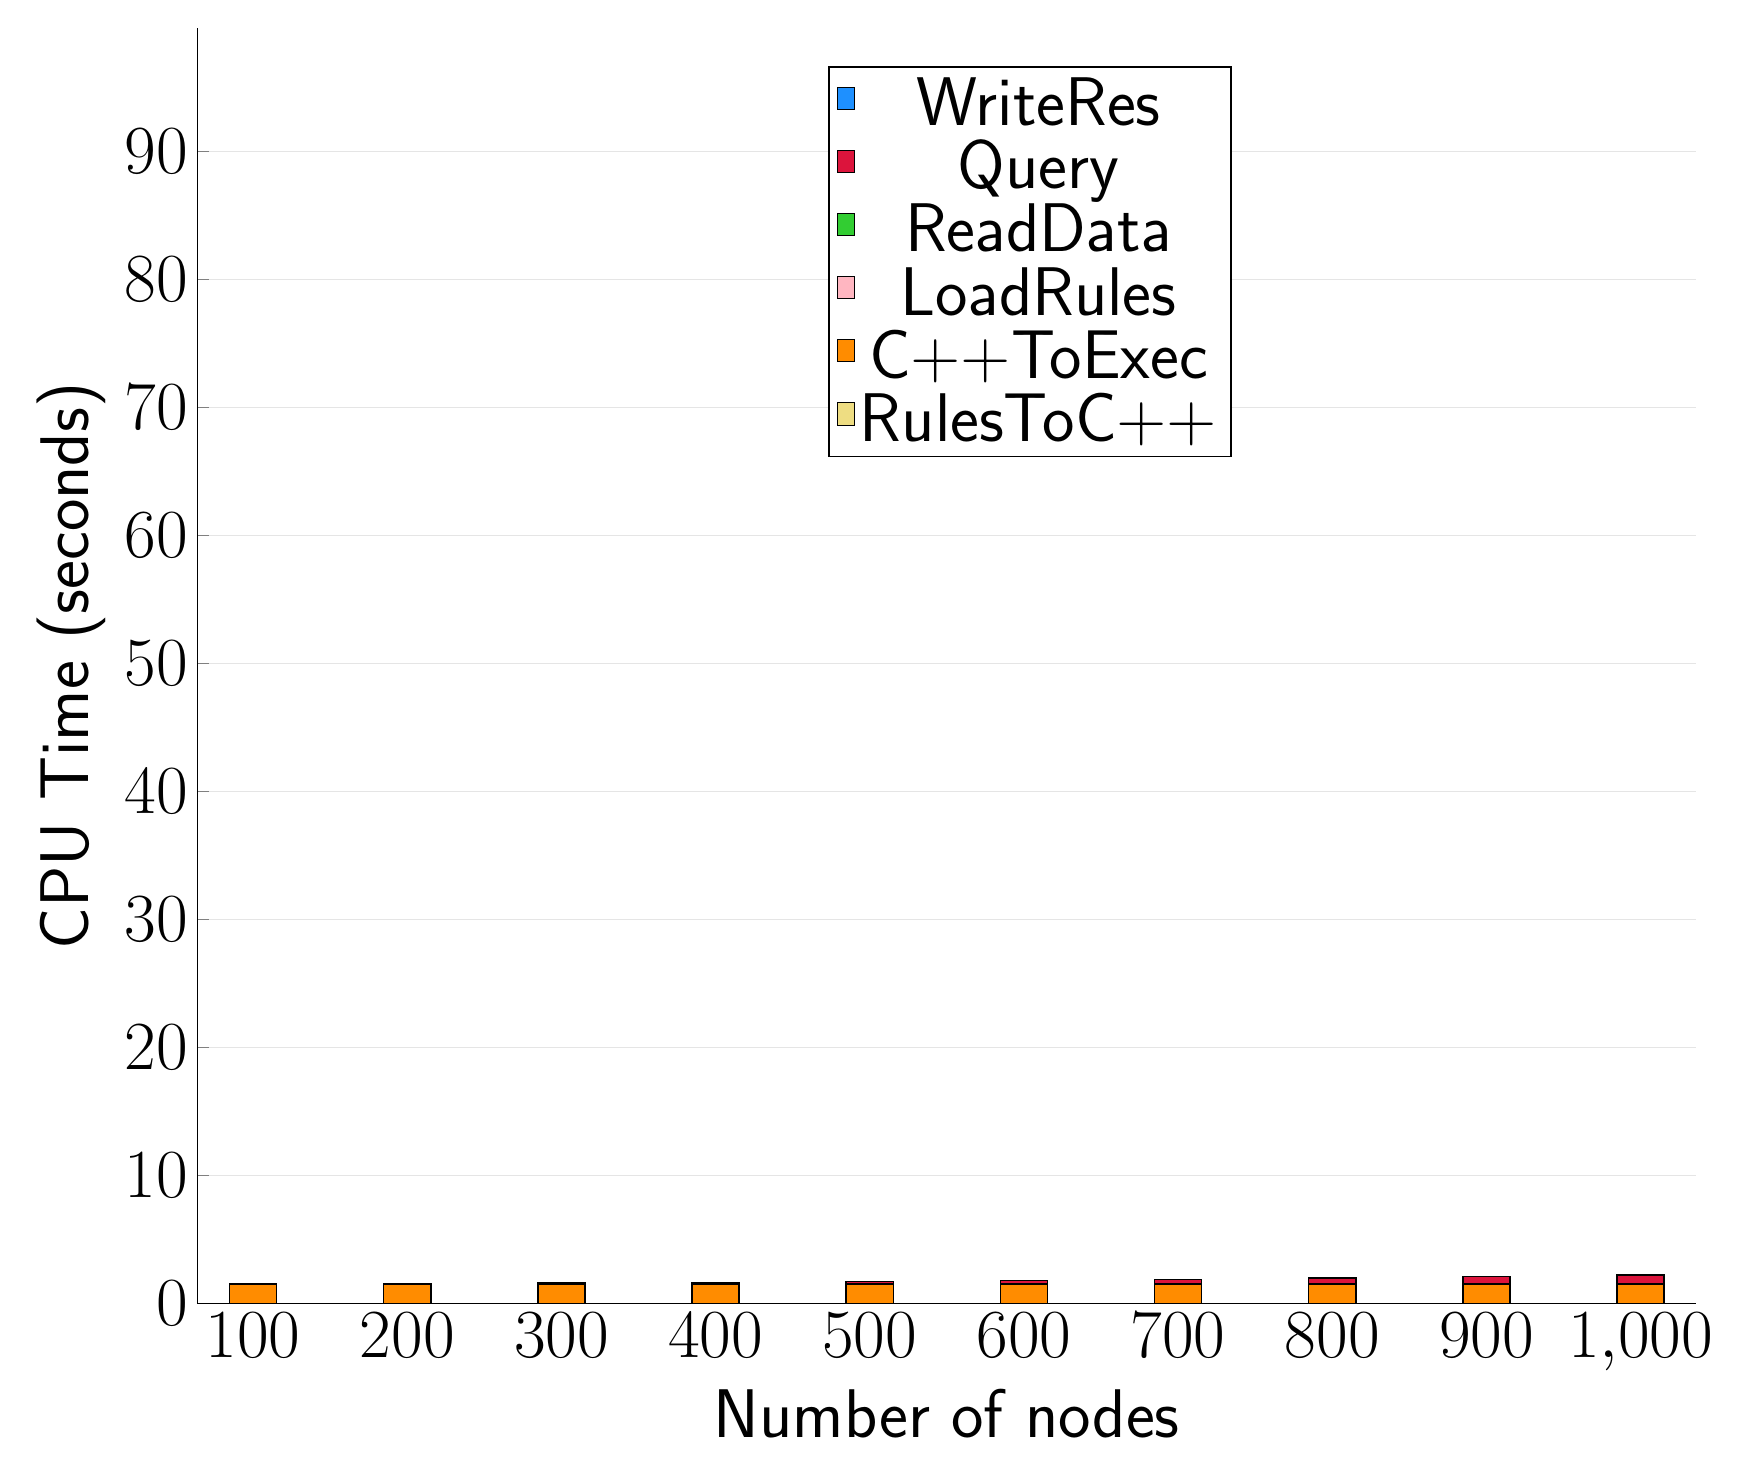
\begin{tikzpicture}
\begin{axis}[
   ybar stacked,
   width=1.7\textwidth,
   bar width=0.6cm,
   ymajorgrids, tick align=inside,
   major grid style={draw=gray!20},
   xtick=data,
   ymin=0, ymax=99.5987,
   axis x line*=bottom,
   axis y line*=left,
   enlarge x limits=0.04,
   legend style={
       at={(0.69, 0.97)},
       anchor=north east,
       legend columns=1,
       font=\Huge,
   },
   ylabel={CPU Time (seconds)},
   xlabel={Number of nodes},
   label style={font=\Huge},
   tick label style={font=\Huge},
]
\addlegendimage{fill=DodgerBlue, draw=black, line width=0.2pt}
\addlegendentry{WriteRes}
\addlegendimage{fill=Crimson, draw=black, line width=0.2pt}
\addlegendentry{Query}
\addlegendimage{fill=LimeGreen, draw=black, line width=0.2pt}
\addlegendentry{ReadData}
\addlegendimage{fill=LightPink, draw=black, line width=0.2pt}
\addlegendentry{LoadRules}
\addlegendimage{fill=DarkOrange, draw=black, line width=0.2pt}
\addlegendentry{C++ToExec}
\addlegendimage{fill=LightGoldenrod, draw=black, line width=0.2pt}
\addlegendentry{RulesToC++}
\addplot +[fill=LightGoldenrod, draw=black, line width=0.55pt] coordinates {
(100, 0.0020000000000000005)
(200, 0.006000000000000001)
(300, 0.004000000000000001)
(400, 0.010000000000000002)
(500, 0.010000000000000002)
(600, 0.006000000000000001)
(700, 0.008000000000000002)
(800, 0.010000000000000002)
(900, 0.008000000000000002)
(1000, 0.008000000000000002)
};
\addplot +[fill=DarkOrange, draw=black, line width=0.55pt] coordinates {
(100, 1.518)
(200, 1.534)
(300, 1.534)
(400, 1.534)
(500, 1.5260000000000002)
(600, 1.532)
(700, 1.528)
(800, 1.532)
(900, 1.5239999999999998)
(1000, 1.52)
};
\addplot +[fill=LightPink, draw=black, line width=0.55pt] coordinates {
(100, 0.0001328)
(200, 0.0001346)
(300, 0.0001406)
(400, 0.00014099999999999998)
(500, 0.0001434)
(600, 0.00015)
(700, 0.0001528)
(800, 0.00015120000000000002)
(900, 0.0001336)
(1000, 0.00015280000000000003)
};
\addplot +[fill=LimeGreen, draw=black, line width=0.55pt] coordinates {
(100, 0.0007908)
(200, 0.0012158)
(300, 0.0016408)
(400, 0.0020354)
(500, 0.0023238)
(600, 0.002796)
(700, 0.0029412)
(800, 0.0034111999999999996)
(900, 0.003481)
(1000, 0.0040644)
};
\addplot +[fill=Crimson, draw=black, line width=0.55pt] coordinates {
(100, 0.011529600000000001)
(200, 0.0408962)
(300, 0.076386)
(400, 0.12183620000000002)
(500, 0.1804504)
(600, 0.2553948)
(700, 0.3442092)
(800, 0.44904099999999997)
(900, 0.5651338)
(1000, 0.7057792)
};
\addplot +[fill=DodgerBlue, draw=black, line width=0.55pt] coordinates {
(100, 0.0002626)
(200, 0.00026199999999999997)
(300, 0.00023799999999999998)
(400, 0.0002372)
(500, 0.0002478)
(600, 0.00027759999999999997)
(700, 0.00029160000000000004)
(800, 0.000341)
(900, 0.0003028)
(1000, 0.00033140000000000003)
};
\end{axis}
\end{tikzpicture}

\end{document}
